% vim: spell
\documentclass{./uafthesis/uafthesis}
% vim: set filetype=tex spell :

\usepackage{amsmath, amssymb, amsfonts} % Thanks, AMS!
\usepackage{xfrac}
\usepackage{graphicx, float} % Graphics stuff
\usepackage{textcomp}
\usepackage{array}
\usepackage{fixltx2e} % Allows \(\) in captions, amongst other things.
\usepackage{pxfonts} % The Paladino font
\usepackage{verbatim}
\usepackage{amsmath}
\usepackage{amssymb,amsfonts,textcomp}
\usepackage{array}
\usepackage{float}
\usepackage[printonlyused,withpage]{acronym}
\usepackage{tocloft}
\usepackage{topsection}
\usepackage{pdflscape}
\usepackage{enumitem}
\usepackage[usenames,dvipsnames]{color}
%\synctex=1
\usepackage[square,numbers,comma,sort&compress]{natbib}

\def\xcolorversion{2.00}

\usepackage[version=latest]{pgf}
\usepackage{xkeyval,calc,tikz,fp}
\usepackage{listings}
\usepackage[textwidth=5em,disable]{todonotes}

%include hyperref last so that it can modify some commands
\usepackage{hyperref}
%add hypcap after hyperref
\usepackage[all]{hypcap}
%include cleverref after hyperref because it says to
\usepackage[noabbrev]{cleveref}

%blue links good for on screen
\hypersetup{linktoc=all,colorlinks,linkcolor=blue,pdfauthor={Jesse Frey},pdfstartview=FitH}
%Black links good for printing
%\hypersetup{bookmarks,colorlinks,citecolor=black,urlcolor=black,filecolor=black,linkcolor=black,pdfauthor={Jesse Frey},pdfusetitle,pdfstartview=FitH}

%add figures folder to graphics path
\graphicspath{{./Figures/}}

%libraries for tikz
\usetikzlibrary{chains}
\usetikzlibrary{decorations.shapes}
\usetikzlibrary{decorations.markings}
\usetikzlibrary{shapes,arrows}
\usetikzlibrary{backgrounds}


%define colors for matlab listings
\definecolor{commentcolor}{RGB}{28,172,0} % color values Red, Green, Blue
\definecolor{stringcolor}{RGB}{170,55,241}

%indent all listings
\lstset{
    xleftmargin=.5in,
    xrightmargin=.5in} 

%setup listings for Matlab for listings
\lstset{language=Matlab,%
    basicstyle=\ttfamily,
    breaklines=true,%
    morekeywords={matlab2tikz},
    keywordstyle=\color{blue},%
    morekeywords=[2]{1}, keywordstyle=[2]{\color{black}},
    identifierstyle=\color{black},%
    stringstyle=\color{stringcolor},
    commentstyle=\color{comentcolor},%
    showstringspaces=false,%without this there will be a symbol in the places where there is a space
    numbers=left,%
    numberstyle={\color{BurntOrange}},% size of the numbers
    numbersep=9pt, % this defines how far the numbers are from the text
    emph=[1]{for,end,break},emphstyle=[1]\color{red}, %some words to emphasise
    %emph=[2]{word1,word2}, emphstyle=[2]{style},    
}




\author{Jesse Frey}
\title{Hardware and Software Implementation of a CubeSat Attitude Determination and Control System}
\degreeyear{2013}
\degreemonth{May}
\degree{Master of Science}
\department{Electrical and Computer Engineering}
%\department{Department of Electrical and Computer Engineering}
%\department{Dept. ECE}
\numberofmembers{3}
\prevdegrees{B.S.}
\college{College of Engineering and Mines}

\gsdean{Dr. John Eichelberger} % the grad school dean's name 
\colldean{Dr. Douglas Goering} % the dean of the college's name 
\depchair{Dr. Charlie Mayer} % the department chair's name
\commchair{Dr. Joe Hawkins} % the committee chair's name

\comone{Dr. Denise Thorsen}
\comtwo{Dr. Dejan Raskovic}

\date{\today}

%make committie lines longer
\committeewidth{4in}


%include defines
% vim: filetype=tex spell

%define some math commands
\newcommand{\vect}[1]{\overrightarrow{#1}}
\newcommand{\cross}[0]{\times}
\newcommand{\matt}[1]{\boldsymbol{#1}}
\newcommand{\transpose}{^T}
\newcommand{\unit}[1]{\, \mathrm{#1}}

%highlight future work
\newcommand{\future}[1]{{\color{red}\itshape#1}}

\pgfdeclareshape{inshape}
{%
  % All anchors are taken from the 'rectangle' shape:
  \inheritsavedanchors[from={rectangle}]%
  \inheritanchor[from={rectangle}]{center}%
  \inheritanchor[from={rectangle}]{north}%
  \inheritanchor[from={rectangle}]{south}%
  \inheritanchor[from={rectangle}]{west}%
  \inheritanchor[from={rectangle}]{east}%
  \inheritanchorborder[from={rectangle}]%
  %
  % Only the background path is different
  %
  \backgroundpath{%
    % First the existing 'circle' code:
    \pgfmathsetlength{\pgf@xb}{\pgfkeysvalueof{/pgf/outer xsep}}%
    \pgfmathsetlength{\pgf@yb}{\pgfkeysvalueof{/pgf/outer ysep}}%
    \ifdim\pgf@xb<\pgf@yb%
      \advance\pgfutil@tempdima by-\pgf@yb%
    \else%
      \advance\pgfutil@tempdima  by-\pgf@xb%
    \fi%
    \pgfpathcircle{\centerpoint}{\pgfutil@tempdima}%
    %
    % Now the | and -- lines:
    \pgfmoveto{\pgfpointadd{\centerpoint}{\pgfpoint{0pt}{\pgfutil@tempdima}}}%
    \pgflineto{\pgfpointadd{\centerpoint}{\pgfpoint{0pt}{-\pgfutil@tempdima}}}%
    \pgfmoveto{\pgfpointadd{\centerpoint}{\pgfpoint{\pgfutil@tempdima}{0pt}}}%
    \pgflineto{\pgfpointadd{\centerpoint}{\pgfpoint{-\pgfutil@tempdima}{0pt}}}%
  }%
}

%set default arrows to stealth
\tikzset{>=latex}
% Define block styles
\tikzstyle{decision} = [diamond, draw, fill=blue!20, text width=4.5em, text badly centered, inner sep=0pt]
\tikzstyle{block} = [rectangle, draw, fill=blue!20, text width=5em, text centered, rounded corners, minimum height=4em]
\tikzstyle{bigblock} = [rectangle, draw, fill=blue!20,rounded corners, minimum height=4em]
\tikzstyle{input} = [rectangle, draw, fill=green!20, text width=5em, text centered, rounded corners, minimum height=4em]
%\tikzstyle{input} = [inshape, draw, fill=green!20, text width=5em, text centered, minimum height=4em]

\tikzstyle{oppr} = [draw, circle,fill=blue!20,minimum height=2em]
\tikzstyle{cloud} = [draw, ellipse,fill=red!20, node distance=3cm,minimum height=2em]
%connections styles for flow charts
\tikzstyle{line} = [draw]
\tikzstyle{conn} = [draw,->]
\tikzstyle{phconn} = [draw,->,dashed]
%connection styles for block diagrams
\tikzstyle{bidr} = [draw,<->]
%\tikzstyle{flow} = [draw,--,decorate,decoration=triangles]
\tikzstyle{flow} = [draw,%
          decoration={%
            markings,%
            mark=at position 0.65 with {\arrow[scale=2]{stealth}},
          },postaction=decorate]
          
%hardware block diagram styles
\tikzstyle{powerL} = [draw,color=red!80,thick,line width=0.5mm]
\tikzstyle{powerB} = [->,ultra thick,draw,color=red!50,line width=0.5mm]
\tikzstyle{dataL} = [draw,color=blue,line width=0.5mm]
\tikzstyle{commandL} = [draw,color=green]
\tikzstyle{power} = [rectangle, draw, fill=red!80!black, text width=5em, text centered, minimum height=4em,on chain]
\tikzstyle{prog} = [rectangle, draw=red!30, fill=red!20,text width=5em,text centered,on chain,node distance=1cm]
\tikzstyle{perif} = [rectangle, draw=green!80, fill=green!40,text centered,on chain]
\tikzstyle{hardware} = [rectangle, draw, fill=blue!20, text width=5em, text centered,minimum height=4em,on chain]
\tikzstyle{CPU} = [draw=black,fill=blue!5,inner sep=0]
\tikzstyle{Bus} = [line width=3mm,draw=blue,arrows={Latex[length=3mm,width=7mm]-Latex[length=3mm,width=7mm]}]
\tikzstyle{PCB} = [rectangle,draw=black,inner sep=5mm]



%point used as a dummy node for complicated arrows
\tikzstyle{point} = [circle,inner sep=0pt,minimum size=0pt,fill=none,node distance = 0.5cm]
%\tikzstyle{point} = [circle,inner sep=0pt,minimum size=2pt,fill=red,node distance = 0.5cm]     %alternate point for debugging

%style for annotating fiugres
\tikzstyle{na} = [baseline=-.5ex,remember picture]

%name of MATLAB
\newcommand{\matlab}{MATLAB\xspace}

%draw cubesat with axes
\newcommand{\cubesat}[2]{
    \draw (#1:#2) node{\pgftext[rotate=#1]{\includegraphics[height=\ARCheight]{cube-icon}}};
    \draw[->,cyan,thick] (#1:#2) -- +(#1+90:\axlen);
    \draw (#1:#2) ++(#1+90:\axlen) node[rotate=#1-90,anchor=south west] {\tiny +Y};
    \draw[->,red,thick] (#1:#2) -- +(#1:\axlen);
    \draw (#1:#2) ++(#1:\axlen) node[rotate=#1-90,anchor=north west] {\tiny -Z};
}

%styles for bias modes
\tikzstyle fieldarrow=[arrows={-Latex[color=blue,fill=red,length=3mm,width=1.5mm]}]  %field arrow style
\tikzstyle bias=[<->,YellowOrange,very thick]                                        %bias arrows style

%field lines for winplace figure
\tikzstyle field=[color=blue,thick,postaction={decorate,decoration={markings,mark=at position .35 with {\arrowreversed[thin]{Latex[length=8mm,width=3mm,fill=red]}}}}]

%rotation arrow style for winplace figure
\tikzstyle motion=[->,Plum,very thick]

%draw magnet
\newcommand{\magnet}{
    %draw magnet
    \fill[color=white] (0.25,0.5) rectangle (-0.25,0);
    \fill[color=red] (0.25,0) rectangle (-0.25,-0.5);
    \draw[color=red] (0, 0.2) node {S};
    \draw[color=white] (0,-0.2) node {N};
    \draw[color=black] (0.25,0.5) rectangle (-0.25,-0.5);
}

%draw magnetic field lines
\newcommand{\fieldlines}{
    \begin{scope}
        \clip (0,0) circle (3cm);

        % Computes a point on a field line given r and t
        \newcommand{\fieldlinecurve}[2]{%
            {(pow(##1,2))*(3*cos(##2)+cos(3*(##2)))*0.7}, {(pow(##1,2))*(sin(##2)+sin(3*(##2)))}%
        }

        \foreach \r in {0.85,0.98,1.3,1.8} {
            \draw[color=blue,smooth,variable=\t, samples at={0,-5,-10,...,-360}] plot (\fieldlinecurve{\r}{\t});
        }

        \draw[fieldarrow] (\fieldlinecurve{0.85}{17}) -- (\fieldlinecurve{0.85}{23});
        \draw[fieldarrow] (\fieldlinecurve{0.98}{23}) -- (\fieldlinecurve{0.98}{28});
        \draw[fieldarrow] (\fieldlinecurve{1.3}{50}) -- (\fieldlinecurve{1.3}{52});
        \draw[fieldarrow] (\fieldlinecurve{1.8}{65}) -- (\fieldlinecurve{1.8}{65.5});

        \draw[fieldarrow] (\fieldlinecurve{0.85}{-23}) -- (\fieldlinecurve{0.85}{-17});
        \draw[fieldarrow] (\fieldlinecurve{0.98}{-28}) -- (\fieldlinecurve{0.98}{-23});
        \draw[fieldarrow] (\fieldlinecurve{1.3}{-52}) -- (\fieldlinecurve{1.3}{-50});
        \draw[fieldarrow] (\fieldlinecurve{1.8}{-65.5}) -- (\fieldlinecurve{1.8}{-65});

        \draw[fieldarrow] (\fieldlinecurve{0.85}{180-17}) -- (\fieldlinecurve{0.85}{180-23});
        \draw[fieldarrow] (\fieldlinecurve{0.98}{180-23}) -- (\fieldlinecurve{0.98}{180-28});
        \draw[fieldarrow] (\fieldlinecurve{1.3}{180-50}) -- (\fieldlinecurve{1.3}{180-52});
        \draw[fieldarrow] (\fieldlinecurve{1.8}{180-65}) -- (\fieldlinecurve{1.8}{180-65.5});

        \draw[fieldarrow] (\fieldlinecurve{0.85}{180+23}) -- (\fieldlinecurve{0.85}{180+17});
        \draw[fieldarrow] (\fieldlinecurve{0.98}{180+28}) -- (\fieldlinecurve{0.98}{180+23});
        \draw[fieldarrow] (\fieldlinecurve{1.3}{180+52}) -- (\fieldlinecurve{1.3}{180+50});
        \draw[fieldarrow] (\fieldlinecurve{1.8}{180+65.5}) -- (\fieldlinecurve{1.8}{180+65});
    \end{scope}
}



\begin{document}

\listoftodos
\clearpage

%highlight overfull Hboxes
%\overfullrule=5pt
\showboxdepth=\maxdimen
\showboxbreadth=\maxdimen

\pagenumbering{Roman}
\setcounter{page}{1}
\thispagestyle{empty}


\phantomsection
%\maksig
\makenamedsig

\phantomsection
\maketitle

\clearpage

\phantomsection
\begin{abstract}
    % vim: filetype=tex spell
%CubeSats are becoming all the rage with universities these days. There small form factor and low mass put restrictions on the mass and power budgets that make the conventional attitude control mechanisms less attractive. Many CubeSats with attitude control use ether active or passive magnetic systems. This thesis describes the implementation of a system that provides better control than passive systems with lower power consumption then active systems.

%Magnetic attitude control for CubeSats comes in one of two forms active or passive. Passive systems use permanent magnets and hysteresis material which draw no power from the CubeSat but the orientation is relative to the local magnetic field. Active systems generally use coils that produce torque only when current is driven through them allowing better control of the attitude of the CubeSat while using more power. The \ac*{ARC} will have an attitude control system that uses coils with a hard magnetic core which allows torque to be generated without a constant expenditure of energy but allows the torque to be changed. To achieve proper attitude alignment a biasing scheme is used which removes the need for absolute attitude knowledge.

%The \acf*{ARC} is a CubeSat which is being built at the \acf*{UAF}. The spacecraft utilizes a unique atitude control system which uses hard magnetic torquers for atitude control. 


%Magnetic attitude control systems fall into two main categories: active and passive. Active control is often achieved by running current through a coil to produce a dipole moment, while passive control uses the dipole moment from permanent magnets that consume no power. This presentation describes a system that uses twelve hard magnetic torquers along with a magnetometer to achieve three-axis attitude alignment. The torquers only consume current when their dipole moment is flipped, thereby significantly reducing power requirements compared with traditional active control.  Final attitude alignment is achieved using a dual axis magnetic dipole moment bias algorithm. The system has been shown, in simulation, to be capable of detumbling and aligning a 1U CubeSat to within 5° of a nadir facing attitude in a high inclination orbit. The presentation will focus on design, testing and fabrication of CubeSat hardware in preparation for a proposed launch in 2013.

In recent years there has been a growing interest in smaller satellites. Smaller satellites are cheaper to build and launch then larger satellites. One form factor, the CubeSat, is especially popular with universities and is a 10~cm cube. Being smaller means that the mass and power budgets are tighter and as such new ways must be developed to cope with these constraints. Traditional attitude control systems often use reaction wheels with gas thrusters which present challenges on a CubeSat. Most CubeSats use magnetic attitude control which uses the Earth's magnetic field to torque the satellite into the proper orientation. Magnetic attitude control systems fall into two main categories: active and passive. Active control is often achieved by running current through a coil to produce a dipole moment, while passive control uses the dipole moment from permanent magnets that consume no power. This thesis describes a system that uses twelve hard magnetic torquers along with a magnetometer. The torquers only consume current when their dipole moment is flipped, thereby significantly reducing power requirements compared with traditional active control. The thesis will focus on design, testing and fabrication of CubeSat hardware and software in preparation for launch.


\end{abstract}

%\clearpage

%Table of Contents and such
\phantomsection
\pdfbookmark[0]{Table Of Contents}{toc}
\tableofcontents

\clearpage

\phantomsection
\listoffigures

\clearpage

%\listofmyequations
%\listoftables

%\clearpage


\phantomsection
\frontchap*{List of Acronyms}
\addcontentsline{toc}{frontchapter}{List of Acronyms}

% vim: filetype=tex spell

\acrodefplural{MEMS}[MEMS]{Microelectromechanical systems}
\acrodefplural{CDS}[CDS's]{CubeSat Design Specifications}

\newacro{CalPoly}[Cal Poly]{California Polytechnic University}
\begin{acronym}[MOSFET]
    \acro{ACS}{Attitude Control System}
    \acro{ADC}{Analog to Digital Converter}
    \acro{ACDS}{Attitude Control and Determination System}
    \acro{ADS}{Attitude Determination System}
    \acro{AMR}{Anisotropic MagnetoResistance}
    \acro{ARC}{Alaska Research CubeSat}
    \acro{ASGP}{Alaska Space Grant Program}
    \acro{BCR}{Battery Charge Regulator}
    \acro{CDS}{CubeSat Design Specification}
    \acro{CDH}{Command and Data Handling}
    \acro{COMM}{Communication System}
    \acro{CRC}{Cyclic Redundancy Check}
    \acro{EMO}{Education Mission Objective}
    \acro{EPS}{Electrical Power System}
    \acro{GPIO}{General Purpose Input/Output}
    \acro{LEDL}{Launch Environment Data Logger}
    \acro{NSF}{National Science Foundation}
    \acro{I2C}{Inter-Integrated Circuit}
    \acro{IMG}{Imaging System}
    \acro{LPMT}{Low Power Magnetic Torquer}
    \acro{MEMS}{Microelectromechanical systems}
    \acro{MOSFET}{Metal Oxide Semiconductor Field Effect Transistor}
    \acro{PCB}{Printed Circuit Board}
    \acro{PPOD}[P-POD]{Poly-Picosatellite Orbital Deployer}
    \acro{RAM}{Random Access Memory}
    \acro{SD}[SD card]{Secure Digital card}
    \acro{SMO}{Science Mission Objective}
    \acro{SPB}{Solar Panel Board}
    \acro{SPI}{Serial Peripheral Interface}
    \acro{SSEP}{Space Systems Engineering Program}
    \acro{USB}{Universal Serial Bus}
\end{acronym}


%\listofothermaterials
%\listofappendices


\begin{acknowledgements}
    %Many people have made this thesis posible. I should give them credit here.

\end{acknowledgements}

\acresetall 
\acused{UAF}

% vim: filetype=tex spell

%Introduction: give background on ARC project

\chapter{Introduction}

This thesis describes a CubeSat attitude control system. The system uses \acfp{LPMT}, which are torquers with a hard magnetic core that can be flipped by pulsing current through a coil that wraps around the core. This allows the system to achieve a nadir facing alignment while using less power than current systems. 

\section{CubeSats}

Over the past few decades electronic, devices have continued to get smaller, cheaper and more powerful. This has made many things possible that were not feasible before. Recently, it has become possible for a large number of universities to build and launch their own small satellites.

The \acf{CDS}\cite{CDS} is a small satellite standard that many universities, private companies and NASA have used to help them put satellites into orbit cheaper and easier than before. The \ac{CDS} defines, among other things, the size of the CubeSats, a 10-cm cube, and how they interface with the launcher. Because CubeSats are small and launched from a standard launcher, they are easy to integrate into the extra space leftover on larger missions making launches relatively cheap and easy to obtain.

In recent years, the number of CubeSat launches has grown significantly. CubeSats are launched by universities as well as government institutions like NASA and the Air Force \todo{find references} and private companies. CubeSats were originally envisioned as an educational tool that would have the approximate capabilities of Sputnik\todo{Saw this at a CubeSat conference, find a suitable reference.}. While CubeSats may have been conceived as primarily an educational tool, \todo{find reference(s)} CubeSats have been the subject of NSF grants \cite{NSFcube}.

\section{CubeSat \acs*{ACDS}}

Because CubeSats are small, they have limited surface area for power generation. Many CubeSats do not use deployable solar panels because of their complexity, volume and weight. The result is that CubeSats have to run on a limited power budget. Many CubeSat science missions require at the very least a stable attitude or a nadir pointing attitude. On larger satellites, reaction wheels and thrusters are often used for attitude control. For many CubeSats, the added mass, power and volume of reaction wheels and thrusters is not a viable option.

One common CubeSat attitude control method is to use the Earth's magnetic field. Magnetic attitude control systems are generally capable of less torque than thrusters and reaction wheels, but are smaller and lighter making them a popular choice for many CubeSats. Because magnetic torquers produce different torque based on the angle between the torquer and the magnetic field, a completely passive system can be built. This is a popular choice for systems that mainly need to be detumbled as it is small, light and simple. 

\subsection{Passive Control}

In a passive system, a permanent magnet on the spacecraft forces an axis to align with the local magnetic field. Because there is little friction in space, additional hysteresis material must be added to the spacecraft to dampen oscillations. The hysteresis material dissipates energy in a changing magnetic field, thereby reducing the angular velocity. The main drawback for a passive system is that there is no face of the satellite that is continually facing the Earth. Having a face that constantly points in the nadir direction is useful for communications and for Earth observation.

\subsection{Active Control}

Active magnetic control allows for different attitude options such as nadir pointing. Many CubeSats use air core magnetic torquers built into the solar panel \ac{PCB} such as in \cite{6511478,ClydePannel}. The coils are made of spiral shaped traces in one or more layers of the \ac{PCB}. To increase efficiency some CubeSats use wire wound torquers with a magnetic core. In both cases, however, torque is generated only when current is flowing through the coil. 

\subsection{\acl*{LPMT} Control}

The system described in this thesis falls somewhere in between passive and active systems. The \acp{LPMT} used in the design allows more control of the attitude than a passive system, yet uses less power than current active systems\todo{Find some good numbers here}. The \ac{LPMT} is a good fit for CubeSats because of its power savings.

\section{\acl*{ARC}}

\ac{ARC} is a CubeSat built by the UAF \ac{SSEP} and funded by \ac{ASGP}. The main purpose of \ac{ARC} is to give students a chance to work on real space flight hardware. The \ac{ARC} has two mission objectives which pertain to the \ac{ACDS} system. The first is to \enquote{Validate a novel low power \ac{ACDS}.}\cite{ARCweb} This will be accomplished by implementing a low power \ac{ACDS} and collecting data on its performance. The second is to \enquote{Validate a high bandwidth communication system by obtaining images of changing snow/ice coverage in arctic regions.}\cite{ARCweb} This will be accomplished by putting the satellite in a nadir facing attitude so the camera takes pictures of the Earth and the communication antenna talks to the ground.

\section{\acl*{ACDS}}

The basic \ac{ACDS} algorithm and torquer specifications have been designed by Dr. Donald Mentch for his doctoral thesis\cite{Mentch11}. The remaining work for this thesis is the design, implementation and testing of the hardware and software to realize the \ac{ACDS} on the \ac{ARC}. In addition some parts of the system have been changed from the way the system was originally proposed due to practical considerations.

\Cref{ch:BG} outlines the previous work on \acp{LPMT} and the alignment algorithm that will be used on the \ac{ARC}.

\Cref{ch:CubeSatHardware} describes how the \ac{ACDS} hardware is implemented on the \ac{ARC}. This hardware was constructed based on the parameters outlined in \cite{Mentch11} but the bulk of the design, implementation and testing, was done by the author of this thesis.

\Cref{ch:Software} describes the software for the \ac{ACDS}. The algorithm for \ac{ACDS} was written by Donald Mentch for his doctoral work \cite{Mentch11}. For this thesis, the algorithm was converted from a \matlab simulation into C code so in order to run on the \ac{ARC} \ac{ACDS} embedded system. Because of the change in platform, many support functions had to be written.

\Cref{ch:Verification} describes the test used to validate the performance of the ACDS hardware and software. Some of the basic ideas of verification were outlined in \cite{Mentch11} as well as conversations with Donald Mentch. Most of the testing and verification has been performed by the author of this thesis and adjusted accordingly.


% vim: set filetype=tex spell :

\chapter{Background}



%% vim: set filetype=tex spell :

\chapter{CubeSat Implementation}

\label{ch:CubeSat}

%ConOps to background

%Tweak wording so kalman filter comes later

%Also move contingency later

%.1 Torquers
%crank said what he wanted. I say what we can have. Talk about firing circuits.
%.2 Measurements
%present analysis of expected accuracy. Requirement to determination rotation rate. Talk about instrumentation to get there. (Kalman optional)

The block diagram for the CubeSat hardware used to implement the \ac{ADCS}. The hardware necessary for the \ac{ADCS} is spread over multiple subsystems of the \ac{ARC}. The \ac{ADCS} board contains the torquers, driving hardware along with the microcontroller which will run the algorithm. There is one two axis magnetometer located on each of the six of the \acp{SPB}. These are used by the \ac{ADCS} to calculate rotation rates and calculate the magnetic dipole moment required to generate the necessary torque. Spreading the magnetometers across all six faces should give some degree of noise immunity and redundancy. The \ac{LEDL} board also contains \ac{MEMS} angular rate sensors as a redundant reading of the rotation rate of the \ac{ARC}. The sensors on the \acp{SPB} are read by the \ac{LEDL} which then forwards the magnetometer and angular rate measurements to the \ac{ADCS}.

\begin{figure}[H]
    \centering
    \includegraphics[width=0.8\textwidth]{Figures/Block}
    \caption{Block Diagram of the CubeSat \acs{ADCS} system}
\end{figure}

\section{Bus Communication}

The subsystems of the \ac{ARC} will communicate with each other using the ARCBus. The ARCBus consists of shared connections between the subsystems to transmit commands and data. The ARCBus will primary used by the \ac{ADCS} to get sensor data from the \ac{LEDL} and send and receive data to the ground station through the COMM system.

\section{Hardware}

\subsection{CubeSat Overview}

\begin{figure}[H]
    \centering
    \includegraphics[width=0.8\textwidth]{Figures/CubeSat-Diagram}
    \caption{Diagram of the \ac{ARC}}
\end{figure}

\begin{figure}[H]
    \centering
    \includegraphics[width=0.8\textwidth]{Figures/cubesat-core}
    \caption{Core Board Stack of the \ac{ARC}}
\end{figure}

\subsection{Torquers}

\subsubsection{Cores}

The torquer cores from \cite{Mentch11} consisted of a large and a small pair in each axis. The torquers consist of a hard magnetic core an electromagnetic coil to flip the core. All torquer cores were the same size, one inch long $\sfrac{1}{16}$th inch diameter rod. The large pair was made of Alnico1 and produced a magnetic dipole moment of $0.022 \unit{A m^2}$. The small pair was proposed to have an inert core with a thin permalloy coating to give it a dipole moment of $0.00011 \unit{A m^2}$.

The torque that the alnico torquers produce is quite small and is already not easy to measure. Because the small torquers are $\sfrac{1}{200}$th the size of the alnico torquers it was determined that these are not feasible to fabricate. To fix this the small torquers was enlarged to 10\% of the size of the large torquers. The switching interval was also reduced to one second. It was also necessary to relax the desired attitude tolerances to accommodate the new setup.

\subsubsection{Drivers}

The schematic to drive a pair of torquers is shown in \autoref{fig:drive}. Each pair of torquers is driven by three complimentary pairs of \acp{MOSFET}.  The \acp{MOSFET} are driven by three pairs of \ac{MOSFET} drivers which are controlled by the \ac{ADCS} microcontroller.

In the idle state all of the \acp{MOSFET} are off and the torquer coils are floating. This prevents changing magnetic fields in the torquers causing current to flow in them. To flip a torquer one end of the torquer is shorted to ground using one of the N-Channel \acp{MOSFET} and the other end is shorted to C1 using one of the P-Channel \acp{MOSFET}. After a short delay the \acp{MOSFET} are switched off and C1 begins to recharge.

\begin{figure}[H]
    \centering
    \includegraphics[width=0.5\textwidth]{Figures/driverSchematic}
    \caption{Torquer Driver schematic}
    \label{fig:drive}
\end{figure}

\subsection{Sensors}

The only sensor called out in \cite{Mentch11} was a magnetometer. The accuracy of the magnetometer was not specified but it needs to be able to determine rotation rates accurately enough for the \ac{ADCS} to work.

\subsubsection{Magnetometer}

The magnetometers on the satellite are Honeywell HMC1052 \ac{AMR} sensors. These sensors use \ac{AMR} elements in a bridge configuration to measure the field in each axis. The HMC1052 is a 2-axis sensor that measures the field in the axis that are parallel to the board that it is mounted on (X and Y). Each face of \ac{ARC} will have a single HMC1052 giving a total of 4 measurements in each axis.

The \ac{AMR} sensors are primarily sensitive to magnetic fields in their sensitive direction but they are also slightly sensitive to magnetic fields in an axis normal to the sensitive direction. The sensor is only sensitive to magnetic fields that are in the film plane, which is the plane that the \ac{AMR} film is deposited in. For the 2-axis HMC1052 this means that both sensors show some sensitivity to fields in both the X and Y axes. The cross axis effect varies from sensor to sensor \todo{Test this} so calibration values must be calculated for each sensor \cite{AN215}.

\autoref{eq:magfull} shows the full equation for the magnetometer. $V_b$ is the bridge voltage that is applied to the sensor. $S_s$ is the sensitivity in the sensitive direction. C and D are the cross field sensitivity and offset values \cite{AN215}.

\begin{equation}
    V_o = V_b \left( \left( S_s \left( 1 + C \cdot H_c^2 \right) H_s \right) + D \cdot H_c \right)
    \label{eq:magfull}
\end{equation}

Because C is small and is multiplied by miligauss squared to get a really small number, it is ignored for the purposes of calibration which results in the simpler \autoref{eq:magcross}.

\begin{equation}
    V_o = V_b \left( \left( S_s H_s \right) + D \cdot H_c \right)
    \label{eq:magcross}
\end{equation}

\autoref{eq:magcross} is useful to determine the voltage that would be produced for a given magnetic field condition, but not terribly useful if the sensor voltages are known but the fields are not. Furthermore the \ac{ADC} reference voltage will be the same as $V_b$ so knowing the bridge voltage is unnecessary\todo[prepend, caption={Elaborate Here?}]{Seems more or less obvious to me and somewhat cumbersome to fully explain}. 
 
\begin{equation}
    H = C_1 \cdot V_x + C_2 \cdot V_y + C_3
    \label{eq:magcal}
\end{equation}

Because $S_s$ and D from \autoref{eq:magcross} are experimentally determined, it is easier to solve \autoref{eq:magcross} for calibration instead. In this case $V_x$ and $V_y$ are the \ac{ADC} values for the x and y axis respectively. $C_1$ and $C_2$ are the sensitivity and $C_3$ is an offset that can come from offsets in the instrumentation or from external offsets such as torquers. This makes the values that the calibration solves for directly usable to calculate magnetic field from \ac{ADC} measurements.

\subsubsection{Magnetometer Calibration}

Magnetometer Calibration consists of finding the coefficients in \autoref{eq:magcal}. To do this the magnetometer is first placed inside the Helmholtz Cage. This allows the field to be set to any value. Furthermore the field can be set under Matlab control so the entire calibration process can run automatically. The calibration program sweeps the field inside the Helmholtz Cage through a predefined sequence and reads the sensor output at each point. 

\autoref{eq:magcal} can be rearranged into matrix form as shown in \autoref{eq:magmat}. Each line in the matrix represents a separate magnetic field measurement. H is the value set by the Helmholtz cage in the sensitive axis . 

\begin{equation}
    \vect{b}=\matt{A} \vect{x} \quad
    \matt{A} =
    \begin{bmatrix}
        {V_x}_1 & {V_y}_1 & 1 \\
        \vdots & \vdots & \vdots\\
        {V_x}_n & {V_y}_n & 1 \\
    \end{bmatrix} \quad
    \vect{x} = 
    \begin{bmatrix}
        C_1 \\
        C_2 \\
        C_3 \\
    \end{bmatrix} \quad
    \vect{b} = 
    \begin{bmatrix}
        H_1 \\
        \vdots \\
        H_n \\
    \end{bmatrix} \quad
    \label{eq:magmat}
\end{equation}

To calculate the calibration values \autoref{eq:magmat} must be solved for $\vect{x}$. In order to get a better calibration value many measurements are taken resulting in an overdetermined system. To solve this system the least squares method is used as shown in \autoref{eq:maglstsq}.

\begin{equation}
    \hat{\vect{x}} = \left(\matt{A} \transpose \matt{A} \right) ^ {-1} \matt{A} \transpose \vect{b}
    \label{eq:maglstsq}
\end{equation}

The least squared solution minimizes the error across all data points. This results in calibration values that minimize error across the range of calibration points that were taken.

\subsubsection{Torquer Calibration}

Because the torquers produce a magnetic field and are in close proximity to the magnetometer the effects of the torquers must be calibrated out. This is possible because the magnetic field of the torquers have a small number of discrete states and these states are fairly repeatable \todo{Test repeatability}

Because the torquer offsets depend on how the torquers and magnetometer(s) are placed, the offsets must be calculated after the satellite has been fully integrated. To calculate the offsets the satellite is placed in the Helmholtz cage and connected to the Helmholtz Cage Computer. A Matlab script is run that runs the calibration procedure for each combination of torquer states to calculate the offset at each state. 

\subsubsection{Calibration Testing}

To test how well the calibration functions a testing script was written. \autoref{fig:tcalTst} shows a plot from the test script. To run the test script the fully integrated satellite is placed in the Helmholtz cage. The script sweeps the magnetic field of the Helmholtz cage through a predefined field sequence taking magnetic field readings at each step. At fixed intervals the satellite is told to flip a random torquer in each axis in a random direction. The previously defined correction data for the torquers is used to compute what the external field is. For comparison the readings are also plotted with just the scale factor correction. The difference in readings is very apparent as can be seen in \autoref{fig:tcalTst}.


\begin{figure}[H]
    \centering
    \includegraphics[width=\textwidth]{Figures/torqueCalTst}
    \caption{Torquer Calibration Test Graph}
    \label{fig:tcalTst}
    \todo[inline]{Repeat with fully integrated satellite as it says in the text.}
\end{figure}

\section{Attitude Determination}

The original design did not use attitude determination to get the satellite into the proper orientation. Instead the rotation rates are used along with the bias windows to get the satellite into the right alignment. The problem is that computing the rotation to the needed accuracy is not a simple process. The original idea was that the rotation rates could be computed directly from magnetic field measurements. A set of magnetometer measurements would be taken each time step to compute the rotation rates. The problem is that to do the rotation rate calculation a derivative is needed. Numerical differentiation is possible but it tends to increase noise by acting as a high pass filter.

The proposed rate determination algorithm also falls short because it does not estimate the full rotation rates. Because the magnetic field is used to determine rotation rates rotations around the magnetic field can not be resolved. This was thought not to be an issue because these rotations are also the kind that can not be corrected for by the torquers but it was shown,in simulation, that removing the component of the rotation rates parallel to the magnetic field caused the CubeSat not to stabilize into the proper alignment. 

To solve both of these problems a Kalman filter is used to estimate both the attitude and the rotation rates using the magnetic field data. The Kalman filter estimates the rates by using the assumed satellite dynamics along with a magnetic field model. The Kalman filter uses the knowledge of the system dynamics to smooth the rate estimates and reduce noise. 



\begin{comment}

\begin{equation}
    F_k = 
        \begin{bmatrix}
              0                &   \hat {\omega} _3 & - \hat {\omega} _2  & \frac{1}{2} & 0           & 0           \\
            - \hat {\omega} _3 &   0                &   \hat {\omega} _1  & 0           & \frac{1}{2} & 0           \\
              \hat {\omega} _2 & - \hat {\omega} _1 &   0                 & 0           & 0           & \frac{1}{2} \\
            0 & 0 & 0 & 0                  & K_1 \hat{\omega}_3 & K_1 \hat{\omega}_2 \\
            0 & 0 & 0 & K_2 \hat{\omega}_3 & 0                  & K_2 \hat{\omega}_1 \\
            0 & 0 & 0 & K_3 \hat{\omega}_2 & K_3 \hat{\omega}_1 & 0                  \\
        \end{bmatrix}
\end{equation}

\begin{equation}
    \Phi \left( t \right) = \matt{I} + \matt{F} t = 
        \begin{bmatrix}
              1                  &   \hat {\omega} _3 t & - \hat {\omega} _2 t  & \frac{1}{2} t & 0             & 0             \\
            - \hat {\omega} _3 t &   1                  &   \hat {\omega} _1 t  & 0             & \frac{1}{2} t & 0             \\
              \hat {\omega} _2 t & - \hat {\omega} _1 t &   1                   & 0             & 0             & \frac{1}{2} t \\
            0 & 0 & 0 & 1                    & K_1 \hat{\omega}_3 t & K_1 \hat{\omega}_2 t \\
            0 & 0 & 0 & K_2 \hat{\omega}_3 t & 1                    & K_2 \hat{\omega}_1 t \\
            0 & 0 & 0 & K_3 \hat{\omega}_2 t & K_3 \hat{\omega}_1 t & 1                    \\
        \end{bmatrix}
\end{equation}

\begin{equation}
    \matt{Q} = Q \matt{I}
\end{equation}

\begin{equation}
    \matt{Q}_k = \int _0 ^ {T_s} \matt{\Phi} \left( \tau \right) \matt{Q} \matt{\Phi} \transpose \left( \tau \right) d\tau = Q \int _0 ^ {T_s} \matt{\Phi} \left( \tau \right) \matt{\Phi} \transpose \left( \tau \right) d\tau
\end{equation}


\begin{equation}
    \matt{Q}_k = Q \int _0 ^ {T_s} \matt{\Phi} \left( \tau \right) \matt{\Phi} \transpose \left( \tau \right) d\tau
\end{equation}

\end{comment}
 
\begin{comment}
\begin{figure}[H]
    \centering
    \includegraphics[width=\textwidth]{Figures/test}
    \todo[inline]{Testing Figure}
    \caption{Test Matlab Figure}
\end{figure}

\end{comment}

% vim: set filetype=tex spell :

%CubeSat Chapter 
\chapter{CubeSat Hardware Implementation}

\label{ch:CubeSatHardware}

\section{CubeSat Architecture}

\todo[inline]{Float section to background?}

The \ac{ARC} uses the same board geometry as the CubeSat Kit\cite{CSK} hardware making it compatible with other CubeSat hardware. The \ac{ACDS} board has a slightly different shape than the standard board shape to accommodate the torquers.

\subsection{Stackup}

\Cref{fig:arcMech} shows the mechanical design of the \ac{ARC}. The design has a central board stack with solar pannels and rails attached to rings that are on the top and bottom of the board stack. The \ac{ACDS} board is located 3rd from the bottom of the stack. This puts it in the center of the board stack. Because the solar cells cover all of the side faces except a small strip in the center this makes the \ac{ACDS} board the only place to put access port connections. The separation switch connections are also located on the \ac{ACDS} board as the separation switch is attached to one of the torquer standoff.

\begin{figure}[!ht]
    \centering
    \begin{minipage}{0.41\linewidth}
        \begin{tikzpicture}[remember picture] 
            \def\sysx{0.8}
            \node[anchor=south west,inner sep=0] (image) at (0,0) {\includegraphics[width=\linewidth]{cubesat-core}};
            \begin{scope}[x={(image.south east)},y={(image.north west)}]
                % define destination coordinates
                \path (\sysx,0.751) coordinate (LEDL)
                      (\sysx,0.633) coordinate (EPS)
                      (0.86,0.55) coordinate (Z1tq)
                      (0.12,0.55) coordinate (Z2tq)
                      (0.3,0.52) coordinate (Xtq)
                      (\sysx,0.465)  coordinate (ACDS)
                      (0.9,0.4)  coordinate (sep)
                      (\sysx,0.366)  coordinate (COMM)
                      (\sysx,0.281)  coordinate (IMG);
              \end{scope}
        \end{tikzpicture}
    \end{minipage}\begin{minipage}{0.42\linewidth}
        \begin{itemize}
            \itemsep-0.7em
            \item[\kern-2em] \tikz[na] \coordinate (LEDLi); LEDL
            \item[\kern-2em] \tikz[na] \coordinate (EPSi); EPS
            \item[\kern-2em] \tikz[na] \coordinate (Ztqi); Z Torquer
            \item[\kern-2em] \tikz[na] \coordinate (Xtqi); X Torquer
            \item[\kern-2em] \tikz[na] \coordinate (ACDSi); ACDS board
            \item[\kern-2em] \tikz[na] \coordinate (sepi); Separation switch
            %\item[\kern-2em] \tikz[na] \coordinate (ppi); Pull Pin
            \item[\kern-2em] \tikz[na] \coordinate (COMMi); COMM
            \item[\kern-2em] \tikz[na] \coordinate (IMGi); IMG
        \end{itemize}
    \end{minipage}

    \begin{tikzpicture}[overlay,remember picture]
            \path[->,red,very thick] (LEDLi) edge (LEDL);
            \path[->,red,very thick] (EPSi) edge (EPS);
            \path[->,red,very thick] (Ztqi) edge (Z1tq);
            \path[->,red,very thick] (Ztqi) edge (Z2tq);
            \path[->,red,very thick] (Xtqi) edge (Xtq);
            \path[->,red,very thick] (ACDSi) edge (ACDS);
            \path[->,red,very thick] (sepi) edge (sep);
            \path[->,red,very thick] (COMMi) edge (COMM);
            \path[->,red,very thick] (IMGi) edge (IMG);
    \end{tikzpicture}
    \caption{The \acs{ARC} mechanical setup}
    \label{fig:arcMech}
\end{figure}

\subsection{Mechanical Considerations}
In addition to the \ac{ACDS} hardware the \ac{ACDS} board also contains the pull pin and USB connection. This is located on the \ac{ACDS} board because it is the only board that can connect to the access port. The pull pin and USB connection connect directly to the header and are not connected to the core \ac{ACDS} hardware. 

The Z-axis torquers are housed inside the standoffs which are located on the four corners of the board. To accommodate the standard board shape has been modified to accommodate the torquers. This is visible in \cref{fig:boardPhoto}. The notches are designed to fit the torque standoffs and help keep them in the proper orientation. The torquers fit into a hole drilled into the standoffs and are held in place with epoxy. 

\begin{figure}[!ht]
    \includegraphics[width=\linewidth]{ACDS-board-photo}
    \caption{The \ac{ARC} \ac{ACDS} board}
    \label{fig:boardPhoto}
\end{figure}

The standard board shape has also been modified to allow the USB connector to be placed closer to the access port so that the USB cable can be easily plugged in. This is also visible in \cref{fig:boardPhoto}.

\subsection{Bus Communication}

The subsystems of the \ac{ARC} will communicate with each other using the ARCBus. The ARCBus consists of shared connections between the subsystems to transmit commands and data. The ARCBus will primary used by the \ac{ACDS} to get sensor data from the \ac{LEDL} and send and receive data to the ground station through the COMM system. Commands are transmited using an \ac{I2C} bus and large blocks of data are sent using a SPI bus which is negotiated using the \ac{I2C} bus.

\section{\acl{ACDS} System Block Diagram}

The block diagram for the CubeSat hardware used to implement the \ac{ACDS}. The hardware necessary for the \ac{ACDS} is spread over multiple subsystems of the \ac{ARC}. The \ac{ACDS} board contains the torquers, driving hardware along with the microcontroller which will run the attitude control algorithm. There is one two axis magnetometer located on each of the six of the \acp{SPB}. These are used by the \ac{ACDS} to calculate rotation rates and calculate the magnetic dipole moment required to generate the necessary torque. Spreading the magnetometers across all six faces should give some degree of noise immunity and redundancy. The \ac{LEDL} board also contains \ac{MEMS} angular rate sensors as a redundant reading of the rotation rate of the \ac{ARC}. The sensors on the \acp{SPB} are read by the \ac{LEDL} which then forwards the magnetometer and angular rate measurements to the \ac{ACDS}.

\begin{figure}[H]
    \centering
    \includegraphics[width=0.8\textwidth]{Figures/Block}
    \caption{Block Diagram of the CubeSat \acs{ACDS} system}
\end{figure}


\section{Torquers}

\Cref{fig:torquers} shows the torquer locations within the \ac{ARC}. The torquers consist of a hard magnetic core surrounded with a coil of wire. There are a total of twelve torquers on the \ac{ARC}, four in each axis. The torquers are flipped using the driving circuit which causes a current pulse to flow through the coil. The driving hardware for the torquers is designed to flip one torquer in each axis every second.

\begin{figure}[!ht]
    \centering
    \begin{minipage}{0.25\linewidth}
        \begin{itemize}
            \itemsep-0.6em
            \item[\kern-0.2em] Magnetometer \tikz[na] \coordinate (MAGi);
            \item[\kern-0.2em] Y torquers \tikz[na] \coordinate (YTi);
            \item[\kern-0.2em] X torquers \tikz[na] \coordinate (XTi);
            \item[\kern-0.2em] Z torquers\tikz[na] \coordinate (ZTi);
        \end{itemize}
    \end{minipage}\begin{minipage}{0.55\linewidth}
        \begin{tikzpicture}[remember picture] 
            \node[anchor=south west,inner sep=0] (image) at (0,0) {\includegraphics[width=\linewidth]{torquers}};
            \begin{scope}[x={(image.south east)},y={(image.north west)}]
                \fill[blue,fill opacity=0.3] (0.722,0.712) -- (0.74,0.709) -- (0.74,0.683) -- (0.723,0.685) -- cycle;
                \path (0.722, 0.7) coordinate (MAG)
                      (0.28,0.49) coordinate (XT)
                      (0.208,0.51) coordinate (YT)
                      (0.1,0.45) coordinate (ZT1)
                      (0.48,0.4) coordinate (ZT2);
              \end{scope}
        \end{tikzpicture}
    \end{minipage}

    \begin{tikzpicture}[overlay,remember picture]
            \path[->,red,very thick] (MAGi) edge (MAG);
            \path[->,red,very thick] (XTi) edge (XT);
            \path[->,red,very thick] (YTi) edge (YT);
            \path[->,red,very thick] (ZTi) edge (ZT1);
            \path[->,red,very thick] (ZTi) edge (ZT2);
    \end{tikzpicture}
    
    \caption{Torquer locations within the \ac{ARC}}
    \label{fig:torquers}
\end{figure}

\subsection{Cores}

The torquer cores from \cite{Mentch11} consisted of a large and a small pair in each axis. The torquers consist of a hard magnetic core an electromagnetic coil to flip the core. All torquer cores were the same size, one inch long $\sfrac{1}{16}$th inch diameter rod. The large pair was made of Alnico1 and produced a magnetic dipole moment of $0.022 \unit{A m^2}$. The small pair was proposed to have an inert core with a thin permalloy coating to give it a dipole moment of $0.00011 \unit{A m^2}$.

The torque that the alnico torquers produce is quite small and is already not easy to measure. Because the small torquers are $\sfrac{1}{200}$th the size of the alnico torquers it was determined that these are not feasible to fabricate. To fix this the small torquers was enlarged to 10\% of the size of the large torquers. The switching interval was also reduced to one second. It was also necessary to relax the desired attitude tolerances to accommodate the new setup.

\subsection{Coils}

The coils used to drive the torquers are made from four layers of 26 AWG wire. The current spike to flip the torquer peaks around 7A which is significantly higher than 26 AWG can handle with continuous current however, because the pulse duration is short it is not a problem.

\subsection{Drivers}

The schematic to drive a pair of torquers is shown in \cref{fig:drive}. Each pair of torquers is driven by three complimentary pairs of \acp{MOSFET}.  The \acp{MOSFET} are driven by three pairs of \ac{MOSFET} drivers which are controlled by the \ac{ACDS} microcontroller.

In the idle state all of the \acp{MOSFET} are off and the torquer coils are floating. This prevents changing magnetic fields in the torquers causing current to flow in them. To flip a torquer one end of the torquer is shorted to ground using one of the N-Channel \acp{MOSFET} and the other end is shorted to C1 using one of the P-Channel \acp{MOSFET}. After a 2ms delay the \acp{MOSFET} are switched off and C1 begins to recharge.

\begin{figure}[H]
    \centering
    \includegraphics[width=0.5\textwidth]{Figures/driverSchematic}
    \caption{Torquer Driver schematic}
    \label{fig:drive}
\end{figure}

\subsection{Torquer Diagnostics}

Comparators are used to detect in flight if the torquers and drivers are functioning properly. One comparator is used to determine if the capacitor is charged and another is used to detect if the capacitor is discharged. The comparators are checked both before and after a torquer flip to see if the capacitor was charged before an attempted flip and discharged after. If the capacitor did not discharge then the torquer did not flip probably because of a bad connection somewhere. This information is logged in flight and can be used on the ground to analyze how well the torquers are working.

\todo[inline]{Need some discussion of what is done with the info but also need to figure out what should be done.}


\section{Sensors}

The only sensor called out in \cite{Mentch11} was a magnetometer. The accuracy of the magnetometer was not specified but it needs to be able to determine rotation rates accurately enough for the \ac{ACDS} to work.

\subsection{Magnetometer}

The magnetometers on the satellite are Honeywell HMC1052 \ac{AMR} sensors. These sensors use \ac{AMR} elements in a bridge configuration to measure the field in each axis. The HMC1052 is a 2-axis sensor that measures the field in the axis that are parallel to the board that it is mounted on (X and Y). Each face of \ac{ARC} will have a single HMC1052 giving a total of 4 measurements in each axis.

\begin{figure}[!ht]
    \centering
    \begin{minipage}{0.35\linewidth}
        \begin{tikzpicture}[remember picture] 
            \node[anchor=south west,inner sep=0] (image) at (0,0) {\includegraphics[width=\linewidth]{SPB}};
            \begin{scope}[x={(image.south east)},y={(image.north west)}]
                \path (0.715,0.74) coordinate (MAG)
                      (0.395,0.72) coordinate (ADC)
                      (0.395,0.65) coordinate (AMP)
                      (0.745,0.525) coordinate (ACC)
                      (0.615,0.58) coordinate (DAT);
              \end{scope}
        \end{tikzpicture}
    \end{minipage}\begin{minipage}{0.30\linewidth}
        \vspace{1em}
        \begin{itemize}
            \itemsep-0.7em
            \item[\kern-0.2em] \tikz[na] \coordinate (MAGi); Magnetometer
            \item[\kern-0.2em] \tikz[na] \coordinate (ADCi); \acs{ADC}
            \item[\kern-0.2em] \tikz[na] \coordinate (AMPi); Amplifier
            \item[\kern-0.2em] \tikz[na] \coordinate (DATi); Data Connector
            \item[\kern-0.2em] \tikz[na] \coordinate (ACCi); Accelerometer
        \end{itemize}
        \vspace{4em}
    \end{minipage}

    \begin{tikzpicture}[overlay,remember picture]
            \path[->,red,very thick] (MAGi) edge (MAG);
            \path[->,red,very thick] (ADCi) edge (ADC);
            \path[->,red,very thick] (AMPi) edge (AMP);
            \path[->,red,very thick] (ACCi) edge (ACC);
            \path[->,red,very thick] (DATi) edge (DAT);
    \end{tikzpicture}
    
    \caption{Reverse side of the Solar Panel Board showing magnetometer}
    \label{fig:SPB}
\end{figure}

The magnetometers are located on the back of the \acs{SPB}, shown in \cref{fig:SPB}. The magnetometer, with surrounding circuitry, is visible on the back of the board as are the ADC and amplifier. An accelerometer is also located on the back of the solar panel board and is used for a different mission objective. The data connector powers the sensors, including a temp sensor (not shown), and provides access to the sensor data.

\subsubsection{Magnetometer Amplifier}

\todo[inline]{This is mostly for my reference. Should it be here?}

The \ac{SPB} also contains an amplifier to amplify the magnetometer signal before it is read by the \ac{ADC}. This allows the output voltage of the magnetometer to fill the input range of the \ac{ADC}. The required range of the magnetometer will be largely dependent on the torquer geometry and could be more then the $\pm$600 mGuass or so of earths field. The amplifier can be used to trade range for resolution depending on what is needed.

The gain for the amplifier can be calculated as follows: If the maximum output range of the sensor is restricted to $\pm$ 4 gauss. With a bridge voltage of 3.3 V and a sensitivity of 1 mV/V/gauss this results in a $\pm$ 13.2 mV voltage swing. The bridge offset is $\pm$ 1.25 mV/V or $\pm$ 4.125 mV. This results in a total possible swing of $\pm$ 17.325 mV. The input voltage range of the \ac{ADC} is $\pm$ 1.65 V. This results in a gain of about 95. 

\subsubsection{Magnetometer \acl{ADC}}

Each magnetometer has its own \ac{ADC} on each \ac{SPB}. The \ac{ADC} used is the LTC2487. The LTC2487 is a 16-bit delta sigma \ac{ADC} that has two differential analog input channels and an \ac{I2C} interface. For a bridge voltage of 3.3V the HMC1052 has a sensitivity 3.3mV/Gauss. If the amplifier gain is 95 this results in a sensitivity of 0.31V/gauss. For a 3.3V reference voltage the \ac{ADC} has a resolution of $25 \mu V$ this results in a resolution of 81 $\mu$Gauss / LSB.

\subsubsection{Magnetometer Operation}
%\subsection{\acs{AMR} Background}

The HMC1052 sensors used on the \ac{ACDS} are \ac{AMR} sensors. They work by having a bridge with 4 elements that all change resistance with the applied magnetic field. The \ac{AMR} sensors are primarily sensitive to magnetic fields in their sensitive direction, ($H_s$), but they are also slightly sensitive to magnetic fields in an axis normal to the sensitive direction, ($H_C$), called the cross axis. The sensor is only sensitive to magnetic fields that are in the film plane of the \ac{AMR} sensor. For the 2-axis HMC1052 this means that both sensors show some sensitivity to fields in both the X and Y axes. The cross axis effect varies from sensor to sensor \todo[disable]{Test this} so calibration values must be calculated for each sensor \cite{AN215}.

\Cref{eq:magcross} shows the simplified equation for the magnetometer as described in \cite{AN215}. $V_b$ is the bridge voltage that is applied to the sensor. $S_s$ is the sensitivity in the sensitive direction. D is the cross field sensitivity offset. The HMC1052 datasheet\cite{HMC1052} mentions that the sensors have a bridge offset. The bridge offset is the sensor output when zero field is applied to the sensor and can be a large as \textpm1.25 Gauss. The bridge represented by $V_{os}$ in \cref{eq:magcross}.

\begin{equation}
    V_s = V_b \left(S_s H_s + D \cdot H_c + V_{os} \right)
    \label{eq:magcross}
\end{equation}
 
The bridge voltages are measured using an \ac{ADC} that uses the bridge voltage as its reference. To take this into account and simplify the equations, the following substitution is made:
\begin{equation}
    V_s'=\frac{V_s}{V_b}
    \label{eq:adcsub}
\end{equation}

\Cref{eq:magcross} is useful to determine the voltage that would be produced for a given magnetic field condition, but not if the sensor voltages are known but the fields are not.

Because the calculated field in the sensitive direction also depends on the field in the cross axis direction, \cref{eq:magcross} was duplicated for the cross field sensor voltage and both equations were solved simultaneously. This resulted in twice as many constants as \cref{eq:magcross}. The voltages $V_s'$ and $V_c'$ are the normalized \ac{ADC} voltages in the sensitive and cross axis respectively. Each of the constants from \cref{eq:magcross} has similar duplicate forms that comes from the extra equation that was used to solve for $H_s$. To distinguish the constants additional subscripts have been added. \Cref{eq:magsolved} shows \cref{eq:magcross} solved for the unknown quantity, $H_s$.

\begin{equation}
    \begin{split}
    H_s = & \frac{V'_s }{{S_s}_s - \frac{D_s \cdot D_c}{{S_s}_c}} - \frac{D_s \cdot  V'_c }{{S_s}_c \cdot {S_s}_s - D_s \cdot D_c}\\
    & {}- \frac{{S_s}_c \cdot {V_{os}}_s  -D_s \cdot {V_{os}}_c}{{S_s}_c \cdot {S_s}_s - D_s \cdot D_c}
    \end{split}
    \label{eq:magsolved} 
\end{equation}

\Cref{eq:magsolved} can be used to calculate the magnetic field from measured voltages, but the relationship between the constants is complex. To simplify \cref{eq:magsolved} the constants can be consolidated to get \cref{eq:magcal}.

\begin{equation}
    \label{eq:magcal}
    \begin{split}
        H_s &= C_1 \cdot V_s' + C_2 \cdot V_c' + C_3\\
        H_c &= C_4 \cdot V_s' + C_5 \cdot V_c' + C_6
    \end{split}
\end{equation}

In this case $V_s'$ and $V_c'$ are the \ac{ADC} values for the cross and sensitive axes, respectively. $C_1$, $C_2$, $C_4$, and $C_5$ are the sensitivity in the sensitive and cross directions and $C_3$ and $C_6$ correct for the bridge offset of the sensor and also compensates for external offsets. These offset values are used to correct for the torquer offsets.

\subsubsection{Magnetometer Calibration}
\label{sec:magcal}

To calibrate the magnetometer, the coefficients in \cref{eq:magcal} must be calculated. The magnetometer is first placed inside the Helmholtz Cage. The field is set under MATLAB control so the entire calibration process can run automatically. The calibration program sweeps the field inside the Helmholtz Cage through a predefined sequence and reads the sensor output at each point. 

The method of least squares is used to solve \cref{eq:magmat} for the coefficients in \cref{eq:magcal}. Each line in the $\matt{A}$ matrix represents a separate magnetic field measurement. $H_n$ is the $n^{\text{\tiny th}}$ value set by the Helmholtz cage in the sensitive axis. 

\begin{equation}
    \label{eq:magmat}
    \begin{split}
    \vect{b}&=\matt{A} \vect{x} \\
    {\text{\raggedright where}} \\
    \vect{b}&= 
    \begin{bmatrix}
        H_1 \\
        \vdots \\
        H_n \\
    \end{bmatrix} \\
    \matt{A}&=
    \begin{bmatrix}
        {V_s}_1 & {V_c}_1 & 1 \\
        \vdots & \vdots & \vdots\\
        {V_s}_n & {V_c}_n & 1 \\
    \end{bmatrix} \\
    \vect{x}&= 
    \begin{bmatrix}
        C_1 \\
        C_2 \\
        C_3 \\
    \end{bmatrix} 
    \end{split}
\end{equation}

The least squared solution minimizes the error across all data points. This results in calibration values that minimize error across the range of calibration points that were taken. This means that the points used to do the calibration should span the range of values that the magnetometer is expected to measure. 

\subsection{\acs{MEMS} Gyros}

For flight a \ac{MEMS} gyro will also be used to sense rotation rates. The \ac{MEMS} gyro does not have that great resolution compared to what can be achieved with the magnetometer \todo{Perhaps should have some sort of evidence for this}. The gyro does, however directly read the rotation rate so it is good for quickly giving a rough idea of the rotation rates of the satellite. If the satellite is rotating fast enough the magnetometer readings will alias and it can appear that the satellite is rotating at a speed that is much less than the actual speed. If the rotation rates are too high for the \ac{MEMS} gyro the output will saturate and while the rotation rates are not measurable a direction and lower bound can be determined.


\section{Embedded System}

At the heart of the \ac{ACDS} is an embedded system. This system is responsible for running the algorithm, taking housekeeping data and, interfacing with the rest of the satellite.

\subsection{Processor}

The processor used for the \ac{ACDS} and all systems on \ac{ARC} is the MSP430f2618. The MSP430 is a microcontroller aimed at low power applications. The MSP430f2618 runs at a maximum speed of 16MHz and has 8kB of RAM and 116kB of flash memory. The MSP430 microcontrollers do not have an external memory bus so there is no good way to add extra memory or program storage. 

\subsection{SD card}

For flight data storage a SD card is used. This is necessary because of the needed space and write times. The internal flash is limited and also needs to be used for program storage making it undesirable for data storage. Furthermore the internal flash can't be read while it is being written. Because the write times for the internal flash are fairly slow this would disrupt the operation of the program and is not desirable except for the occasional data writes.

\subsection{\acs{ARC} Bus Communication}

The sensor data is read by the \ac{LEDL} board and sent over the bus to the \ac{ACDS} board. The \ac{ACDS} board initiates the connection by sending a command to tell how often measurements should be sent. The \ac{LEDL} then takes sensor data and sends it at the requested interval.

\section{Board Layout}

\Cref{fig:3dview} shows the \ac{ACDS} system. The X and Y axis torquers are shown on the board as well as the pull pin and header. The header and pull pin locations are more or less fixed which doesn't leave much wiggle room for where to place the torquers.

\begin{figure}[H]
    \centering
    \includegraphics[width=0.8\textwidth]{board-drawing}
    \caption{3D view of the CubeSat \acs{ACDS} system}
    \label{fig:3dview}
\end{figure}

\begin{comment}
\begin{figure}[H]
    \centering
    \includegraphics[width=0.8\textwidth]{board-drawing-with-standoffs}
    \caption{3D view of the CubeSat \acs{ACDS} system with Z-axis torquers}
\end{figure}
\end{comment}

\begin{comment}

The \ac{ACDS} board is a four layer board with the inner layers as power and ground planes. \Cref{fig:layout} shows the \ac{PCB} layout for the \ac{ACDS} board. The circuitry is very repetitive and this was used when the board was laid out. A quick switching time is desired and moderate currents are involved, the lines to and from the \acp{MOSFET} were kept as short as possible. The power plane is split so that there is a 3.3V plane underneath the MSP430 and a $V_{batt}$ plane elsewhere.

\begin{figure}[H]
    \centering
    \includegraphics[width=0.8\textwidth]{board-design}
    \caption{Board Layout for the CubeSat \acs{ACDS} system}
    \label{fig:layout}
\end{figure}

\end{comment}

%% vim: set filetype=tex spell :

\chapter{Hardware}

\label{ch:Hardware}

\section{MSP430}

The MSP430 is at the 

\section{Data Storage}

\section{Torquers and Driving Circuit}

\subsection{Mechanical Considerations}

\section{Board Layout}

\begin{figure}[H]
    \centering
    \includegraphics[width=0.8\textwidth]{board-design}
    \caption{Board Layout for the CubeSat \acs{ADCS} system}
\end{figure}

\begin{comment}

\section{Board Renderings}

\begin{figure}[H]
    \centering
    \includegraphics[width=0.8\textwidth]{board-drawing}
    \caption{3D view of the CubeSat \acs{ADCS} system}
\end{figure}

\begin{figure}[H]
    \centering
    \includegraphics[width=0.8\textwidth]{board-drawing-with-standoffs}
    \caption{3D view of the CubeSat \acs{ADCS} system with Z-axis torquers}
\end{figure}

\end{comment}

% vim: filetype=tex spell

\chapter{Software}
\label{ch:Software}

The main responsibility of the \ac{ACDS} software is to determine which torquer to flip each time step. The \ac{ACDS} also needs to keep track of ``house keeping'' information, sensor readings, torquer states and internal control system states so that the performance of the algorithm can be tracked on the ground. 

\section{Overview}

In order to determine which torquer to flip the \ac{ACDS} needs sensor inputs. The sensors are read by the \ac{LEDL} board and forwarded to the \ac{ACDS} using the \ac{ARC}bus. The \ac{ACDS} needs to communicate with the \ac{COMM} board to respond to ground station commands and downlink housekeeping data.

\begin{figure}[H]
    \centering
    %separator for parallel lines
    \def\linesep{6}
    \begin{tikzpicture}[node distance = 3cm, auto]
        % Place nodes
        \node [block,minimum height=8cm]            (AB) {\acs{ARC}bus interface};

        \node [block,left of=AB,node distance=6cm]  (LEDL) {\acs{LEDL}};
        \node [block,left of=AB,yshift=-3cm]        (CDH) {\acs{CDH}};
        \node [block,left of=CDH]                   (COM) {\acs{COMM}};

        \node [bigblock,right of=AB,node distance=7cm,minimum height=5cm,yshift=1.5cm] (core) {\acs{ACDS} software};
        \node [bigblock,below of=core,node distance=4.5cm,minimum height=2cm] (HC) {House Keeping};


        \path [flow] (AB.58) -- node  {Sensor Data} (core.170);
        \path [flow] (core.190) -- node {Sensor Commands} (AB.48);

        \path [flow] (AB.00) -- node {Ground Station} node [below]{Commands} (core.226);

        \path [flow] (core) -- (HC);
        \path [flow] ([yshift= \linesep]AB.290)  -- node [above]{Data Log Query} ([yshift= \linesep]HC.west);
        \path [flow] ([yshift=-\linesep]HC.west) -- node [below]{Recalled Data} ([yshift=-\linesep]AB.290);

        \path [flow] ([yshift= \linesep]COM.east) -- ([yshift= \linesep]CDH.west);
        \path [flow] ([yshift=-\linesep]CDH.west) -- ([yshift=-\linesep]COM.east);

        \path [flow] ([yshift= \linesep]CDH.east) -- ([yshift= \linesep]AB.250);
        \path [flow] ([yshift=-\linesep]AB.250)   -- ([yshift=-\linesep]CDH.east);

        \path [flow] ([yshift=-\linesep]LEDL.east) -- node [below]{Sensor Data}     ([yshift=-\linesep]AB.west);
        \path [flow] ([yshift= \linesep]AB.west)   -- node [above]{Sensor Commands} ([yshift= \linesep]LEDL.east);


    \end{tikzpicture}
    \caption{\acs{ACDS} software overview}
\end{figure}

\section{System Operations Overview}

The \ac{ACDS} starts running after the separation switch is switched and the power system applies power to all systems. Before starting any operations the \ac{ACDS} waits for the on command from the \ac{CDH} board. After the \ac{ACDS} board receives the on command the \ac{ACDS} sends a command to the \ac{LEDL} board to tell it to start taking sensor data. Once sensor data is received the \ac{ACDS} starts to run the detumble algorithm.


\subsection{Ground Station Commands}

The ground station can force the \ac{ACDS} into any mode and ether let it go with the normal flow or stay in a particular mode. This allows for recovery in case the system does not function as expected.

\subsection{Rotation Runaway}

If the gyros detect that the satellite is rotating too fast then they will automatically send the \ac{ACDS} into a safe mode where the \ac{ACDS} does not run. It is possible that the \ac{ACDS} could get into a situation where the algorithm speeds up the rotation instead of slowing it down. In this situation the best thing to do is for the \ac{ACDS} to stop and wait for further intervention from the ground.

\section{Incoming Commands\textbackslash Info}

The \ac{ACDS} must respond to incoming commands that change its operation mode or uplink data. Because the \ac{ACDS} is an experimental system, it may run into unexpected problems. By uplinking commands some of the possible problems can be fixed in flight. 

\begin{comment}
\begin{itemize}
    \item Ground Station Commands
        \begin{itemize}
            \item Uplink Orbit Data
            \item Stop \ac{ACDS}
            \item Force Mode
        \end{itemize}
    \item Sensor Data
\end{itemize}
\end{comment}

\section{Algorithm Software}

\Cref{fig:swblock} shows the overall software block diagram for the \ac{ACDS} system. Field measurements from the magnetometer are calibrated using the current torquer state and a table of field measurements at different torquer states. The calibrated readings are used to calculate rotation rate and latitude which a long with the field readings are used to calculate the torque that should be applied to the satellite. The torque is then quantized based on \cref{fig:lpmtq}. The torquers to flip are chosen based current knowledge of torquer stated as well as the desired torque.

\begin{figure}[H]
    \centering
    \begin{tikzpicture}[node distance = 2.6cm, auto]
    % Place nodes
    \node [block] (field) {Magnetic Field Measurements};
    \node [block,right of=field] (cal) {Torquer offset correction};
    \node [block, right of=cal] (alg) { $C {\dot{\vect{B}}}$ };
    \node [block, right of=alg] (q) {Torque Quantization};
    \node [block, right of=q] (choose) {Choose Torquers to fire};
    \node [point, right of=choose] (fb) {};
    \node [block, right of=fb,node distance=1.5cm] (fire) {Fire Torquers};
    \node [block, below of=choose] (mem) {Torquer Status Tracking};
    \node [block, below of=fire] (sens) {Torquer feedback};

    %draw lines
    \path [conn] (field) -- (cal);
    \path [conn] (cal) -- (alg);
    \path [conn] (alg) -- (q);
    \path [conn] (q) -- (choose);
    \path [conn] (choose) -- (fire);

    \path [conn] (fb) |- (mem.10);
    \path [phconn] (fire) -- (sens);

    \path [conn] (sens.190) -- (mem.350);
    \path [conn] (mem) -- (choose);
    \path [conn] (mem) -| (cal);

    \end{tikzpicture}
    \caption{Overall Software Block Diagram}
    \label{fig:swblock}
\end{figure}

\subsection{B-dot Algorithm}

\label{sec:bdot-desc}

The B-dot algorithm is used to detumble the \ac{ARC}. The B-dot algorithm uses the time derivative of the magnetic field, $\dot{\vec{B}}$, to calculate the magnetic dipole moment that the torquers should generate. This is a method that is widely used on other CubeSats \todo{Find some B-dot reference(s)} that have magnetic \ac{ACDS}. In this mode the magnetic dipole moment is simply set to a value that is proportional to the derivative of the magnetic field. The gain for the B-dot controller needs to be negative in order to stop the motion of the magnetic field. This could be done by adding a negative sign to the torque expression but, in code, it is simpler to have a negative gain.

\section{Auxiliary Software Functions}

In addition to the algorithm software the \ac{ACDS} also requires some auxiliary software to function. In order to generate the proper dipole moment the status of the torquers must be tracked in software so that the right torquer can be flipped. The torquer status also needs to be tracked so that the torquer offsets can be subtracted from the magnetometer measurements. 

\subsection{Torquer Flipping Logic}

The torquer flipping logic keeps track of the torquer status and sets the torquers to the dipole moment that is closest to the dipole moment requested by the control algorithm. The torquer flipping logic also attempts to distribute the flips somewhat evenly across the torquers in any given axis. This way if there are any degradation effects, in the torquer field or the hardware, they will be minimized. 

\subsubsection{Status Tracking}

The status of each torquer is tracked by the flipping logic. This includes flags to indicate if each torquer has been flipped and has had errors being flipped. The last four torquers that were flipped are also tracked. This is used to chose which torquer to flip.

When it is time to flip a torquer the software looks at the current torquer status to figure out which direction a torquer needs to be flipped in. Next the software looks for the torquer that can be flipped in that direction that was flipped the least recently and flips it. This way the torquer flips are distributed across the torquers in a given axis. If torquers are marked as uninitialized then they are flipped first before other torquers so that all torquers are in a known state as quickly as possible.

\subsubsection{torquer feedback}

Before and after each torquer flip the torquer feedback comparators are read. After the torquer flip is complete the feedback values are examined to determine if the torquer flipped. If the capacitor voltage was below the upper threshold before the flip then an error is flagged in the torquer status indicating that there is a problem with the capacitor. If the capacitor voltage after a flip is not below the lower threshold then there is likely a bad connection to the torquer windings. Torquers that failed to flip are flagged and not flipped in the future. It is possible that the comparator could malfunction and indicate that it is both above the upper threshold and below the lower threshold in this case a flag is set to indicate the error and the torquer is assumed to have flipped as normal.

\subsection{Torquer Compensation}

Because the geometry of the system should not change in flight, the field offset seen by each magnetometer depends on the combination of torquer states. By taking measurements in the Helmholtz cage these offsets can be calculated and eliminated during flight in order to measure Earth's magnetic field.

\subsubsection{Compensation Data Set}

\label{sec:comp-dat-set}

There are a total of 12 \acp{LPMT} on the \ac{ACDS}. Each \ac{LPMT} has two states which results in a total of 4096 possible states. If the offset for each state uses four bytes this results in a data set that is 16kB. The field produced at each state however, is the sum of the field contributions of all of the torquers. The dataset can be reduced by doing three separate calibration, one for the set of torquers in each axis. The calibrations are then combined to get a calibration set where one offset is chosen for each axis and added together to get the full offset this reduces the number of states to $3*16 + 1 = 49$ which is only about 200 bytes of data, much reduced from using all possible states.

\subsubsection{Compensation Routine}

\label{sec:tq-comp}

To calculate the compensation values for the torquers the calibration procedure described in \cref{sec:magcal} is run for each combination of torquer states. The results of the compensation is $C_1$, $C_2$, $C_4$ and $ C_5$ which are the same calibration constants computed with the magnetometer calibration routine. In addition there is one common pair of offsets and then 3 sets of 16 offsets for each set of torquers. The total offset value for a given torquer state is the sum of the common offset value and an offset determined by the state of the torquers in the X, Y and Z axes.

\subsection{Data Logging}

During \ac{ACDS} operations data is collected during flight. This data is stored in nonvolatile memory and can be recalled and transmitted to the ground in order to evaluate the \ac{ACDS} system performance. The data that is recorded is shown in \cref{tab:logdat}

\begin{comment}
\begin{itemize}
    \item magnetometer and gyro readings
    \item torquer status
    \item mode
    \item algorithm intermediate results
    \item torquers flipped
    \item torquer feedback
    \item Kalman filter status
    \item Kalman filter internal variables
    \item Kalman filter state
    \item \todo[inline]{More?}
\end{itemize}
\end{comment}

\begin{table}[H]
    \centering
    \caption{\ac{ACDS} operations data format}
    \label{tab:logdat}
    \begin{tabular}{|l|c|c|}
        \hline
        Data&size (bits)&Format\\
        \hline
        mode&2&unsigned integer\\
        \hline
        Time Stamp&32&unsigned integer\\
        \hline
        torquer status&48&flags\\
        \hline
        magnetometer readings&48&unsigned integer (one per axis)\\
        \hline
        gyro readings&36&unsigned integers (one per axis)\\
        \hline
        algorithm intermediate results&TBD&\\
        \hline
        torquers flipped&48&unsigned integer (one per axis)\\
        \hline
        torquer feedback&12&flags\\
        \hline
        Kalman filter status&TBD&\\
        \hline
        Kalman filter internal variables&TBD&\\
        \hline
        \multicolumn{1}{|r|}{\bfseries Total :}&TBD&\\
        \hline
    \end{tabular}
    \todo[inline]{Resolve DBD's}
\end{table}

\subsection{On Board data processing}

Because the downlink data speed is limited, it is necessary to reduce the data that needs to be downlinked. One way to do this is to do some level of on board processing to reduce the data before it is downlinked. For the \ac{ACDS} system this will most likely take the form of returning only the desired data from the recorded data set or returning min/max values from within a data set. 

\subsection{Beacon Data}

The beacon data is transmitted at a fixed rate and provides information about the present state of the satellite. The beacon data could be the only data that is available to diagnose the system. The beacon data must contain enough data to be useful but not so much data that the beacon packets are too big. The beacon data should include raw sensor information as well as information on torquer status. The beacon data from the \ac{ACDS} is shown in \cref{tab:beacondat}

\begin{table}[H]
    \centering
    \caption{Beacon Data format}
    \label{tab:beacondat}
    \begin{tabular}{|l|c|c|}
        \hline
        Data&size (bytes)&Format\\
        \hline
        current magnetometer readings&6&signed integers (one per axis)\\
        \hline
        Mode&1&unsigned integer\\
        \hline
        current torquer status&3&flags\\
        \hline
        number of torquer flips so far & 6 & unsigned integers (one per axis)\\
        \hline
        Kalman filter attitude&8&integer quaternion\\
        \hline
        Kalman filter rates&6&integer vector\\
        \hline
        \multicolumn{1}{|r|}{\bfseries Total :}&30&\\
        \hline
    \end{tabular}
\end{table}


% vim: set filetype=tex spell :

\chapter{Verification}

\label{ch:Verification}

The \ac{ACDS} consists of experimental hardware controlled by experimental software and as such requires a significant amount of verification to make sure everything functions on orbit.

\section{Sensor Verification}

\subsection{Magnetomitor Verification}

The magnetomitor verification is done using the Hemholtz cage 
jj
\subsection{Compensation Testing}

The torquer compensation is tested by running the Helmholtz Cage through a field sequence and taking measurements at each point. During the process a random torquer flip is executed every 10 data points. The measurements are corrected using the compensation data set and compared to the expected field. A typical plot of the data is shown in \cref{fig:tqtst}. The RMS error is also calculated for the data set so the effectiveness of the torquer compensation can be compared to the calibration without torquers.

\begin{figure}[!ht]
    \centering
    \includegraphics[width=0.8\linewidth]{torqueCalTst}
  \caption{A torquer compensation test showing that the correction provides a large amount of improvement over the uncorrected values}
    \label{fig:tqtst}
\end{figure}

\Cref{fig:tqerr} shows the error for the torquer compensation test. The RMS error for the compensated data is 9 mGauss. The maximum error is 24 mGauss. On a 300 mGauss field a 24 mGauss error will cause an angular error of \textpm5\textdegree. The addition of the torquers causes an increase in the RMS and maximum error.
%This can be seen by comparing \cref{fig:tqerr} with \cref{fig:magerr}. In \cref{fig:tqerr} steps in the error are seen as torquers are flipped whereas in \cref{fig:magerr} the error is more consistent across the entire run.

\begin{figure}[!ht]
    \centering
    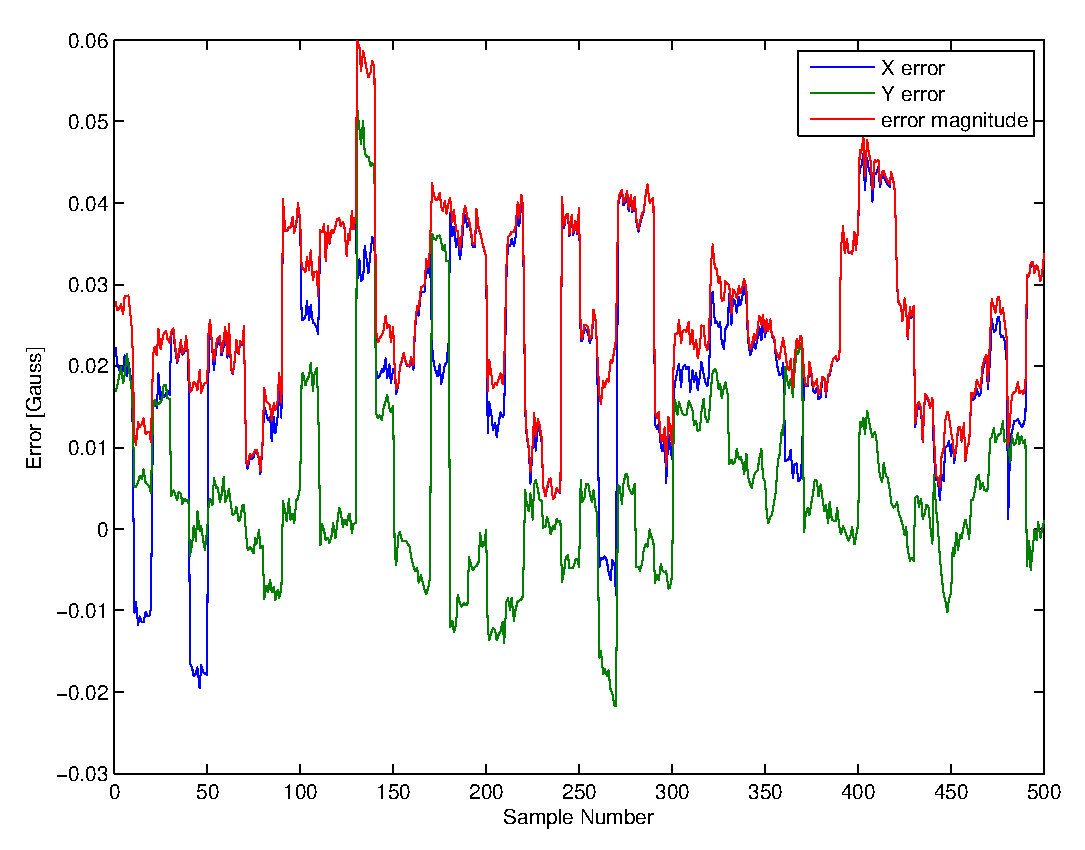
\includegraphics[width=0.8\linewidth]{torqueCalTst-err}
    \caption{Graph showing a torquer compensation error plot}
    \label{fig:tqerr}
\end{figure}

\subsection{Torquer Repeatability}

The torquer compensation method depends on the torquer offsets being repeatable. If the offsets are not very repeatable then the offsets will induce errors in the measured field. \Cref{fig:tqoff} shows a plot of the torquer offsets. The plot shows the offsets of the torquers when they are polarized in each direction. The offset for both of the magnetometer axes are shown. To create the plot each torquer was flipped 20 times in each direction. After each flip a magnetometer calibration was done to get the offset values. The offset values are normalized to show deviation from the median for better comparison. The maximum offset variation in \cref{fig:tqoff} is 20 mGauss.

The offset variations shown in \cref{fig:tqoff} are all less than the maximum error from \cref{fig:tqerr}. This is likely because the maximum offsets did not occur all at the same time.

\begin{figure}[!ht]
    \centering
    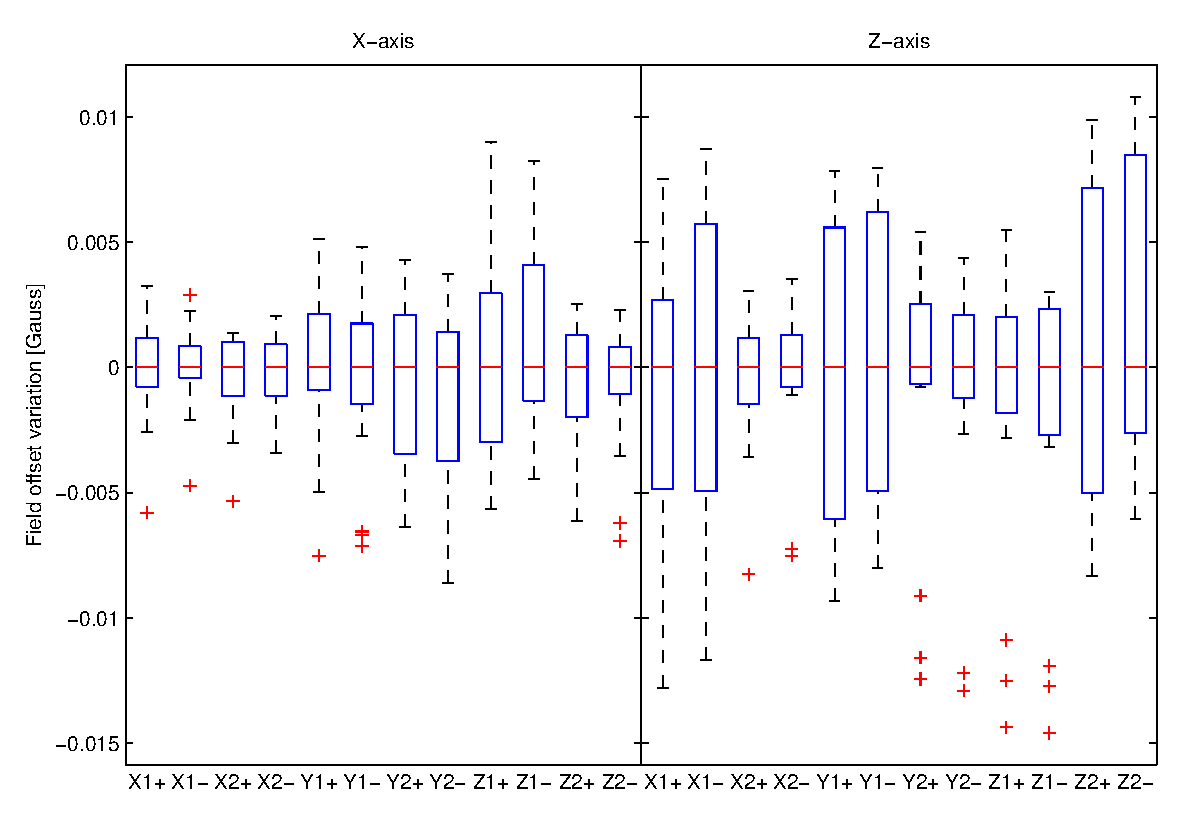
\includegraphics[width=0.9\linewidth]{torqueOffsets}
    \caption{Box Plot from torquer offset test}
    \label{fig:tqoff}
\end{figure}



\subsection{Gyro Verification}

\subsection{Feedback Verification}

To test the torquer feedback 

\section{\acl{ADS} Verification}

\section{Torquer Verification}

\subsection{Driver Verification}

To test the torquer drivers 


\section{Software Verification}

\section{System Verification}

Testing of torquer calibration

Magnetic interference from currents


% vim: filetype=tex spell

\chapter{Conclusion and Future work}

\section{Conclusion}

\section{Future Work}

\subsection{System Operations Overview}

\Cref{fig:sysopflow} shows the system operations flow. The code starts running after the separation switch is switched and the power system applies power to all systems. Before starting any operations the \ac{ACDS} waits for the on command from the \ac{CDH} board. After the \ac{ACDS} board receives the on command the \ac{ACDS} sends a command to the \ac{LEDL} board to tell it to start taking sensor data. Once sensor data is received the \ac{ACDS} starts to run the detumble algorithm. The Kalman filter needs to know the location of the satellite for it to operate properly so orbital elements must be uploaded before the Kalman filter can start running. Once the Kalman filter knows the location of the satellite it still needs some time to converge to a solution. During this time the \ac{ACDS} remains in detumble mode even if the rates have slowed enoughs to exit. Once the Kalman filter is locked and the rates have sufficiently slowed the \ac{ACDS} switches into mode 2. Mode two is run for a set number \todo{figure out how many and put the number here} of orbits (measured by timing). After mode 2 is complete Mode 3 starts. The \ac{ACDS} remains in mode 3 indefinably unless one of undesirable conditions is detected, see \cite{Mentch11} for details, which causes the \ac{ACDS} to attempt to kick the satellite out of the undesirable alignment and then re-stabilize by transitioning back to mode 2.

\begin{figure}[H]
    \centering
    \begin{tikzpicture}[node distance = 0.5cm, auto]
    % Place nodes
    \node [block] (sep) {Separation};
    \node [block,below=of sep] (cmd) {On Command from \acs{CDH}};
    \node [block,below=of cmd] (sens) {Send Start Data Collection Command to \acs{LEDL}};
    \node [block,node distance= 2cm,right=of sep] (detumble) {Detumble};
    \node [decision,below=of detumble] (dchk) {Rates and Kalman filter are ready};
    \node [block,below=of dchk] (m2) {Mode 2};
    \node [decision,below=of m2] (m2chk) {Has Mode 2 time elapsed?};
    \node [block,below=of m2chk] (m3) {Mode 3};
    \node [decision,below=of m3] (cchk) {Correct Alignment?};
    \node [block,node distance=2cm,right=of cchk]  (cor) {apply correction};
    \node [block,above=of cor]  (timer) {reset Mode 2 timer};

    \path[conn] (sep) -- (cmd);
    \path[conn] (cmd) -- (sens);
    \path[conn] (sens.east) -- ++(0.5cm,0) |- (detumble);

    \path[conn] (detumble) -- (dchk);
    \path[conn] (dchk) --  node [near start] {yes} (m2);
    \path[conn] (dchk.east) -- node [near start] {no} ++(0.7cm,0) |-  (detumble);
    \path[conn] (m2) -- (m2chk);
    \path[conn] (m2chk) -- node [near start] {yes} (m3);
    \path[line] (m2chk.east) -- node [near start] {no} ++(0.7cm,0) |- (m2);

    \path[conn] (m3) -- (cchk);
    \path[conn] (cchk) -- node [near start] {no} (cor);
    \path[conn] (cor) -- (timer);
    \path[conn] (timer) |- (m2);

    \path[conn] (cchk.west) -- node [near start] {yes} ++(-0.7cm,0) |- (m3);

    \end{tikzpicture}
    \caption{System operations chart}
    \label{fig:sysopflow}
\end{figure}

The flow case the flow from \cref{fig:sysopflow} can be disrupted. This can happen due to commands from the ground station or if the gyros detect that the sattelite is rotating too fast. The ground station can force the \ac{ACDS} into any mode and ether let it go with the normal flow or stay in a particular mode. This allows for recovery in case the system does not function as expected.

If the gyros detect that the satellite is rotating too fast then they will automatically send the \ac{ACDS} into a safe mode where the \ac{ACDS} does not run. It is possible that the \ac{ACDS} could get into a situation where the algorithm speeds up the rotation instead of slowing it down. In this situation the best thing to do is for the \ac{ACDS} to stop and wait for further intervention from the ground.

\subsubsection{Additional Ground station Commands}

In order for the Kalman filter to work it needs the orbital elements for the satellite. These must be uplinked from the ground because they change as the orbit decays. In addition gains for the control algorithm and Kalman filter may need to be changed in flight to account for unexpected conditions. 


\begin{figure}[H]
    \centering
    \begin{tikzpicture}[node distance = 0.5cm, auto]
    % Place nodes
    \node [block] (field) {Magnetic Field Measurements};
    \node [block,right=of field] (cal) {Torquer offset correction};
    \node [block,node distance=0.7cm,right=of cal] (alg) {Torque algorithm};
    \node [block, right=of alg] (q) {Torque Quantization};
    \node [block, above=of alg] (rates) {Kalman Filter};
    \node [block,above=of cal] (igrf) {Magnetic field model};
    \node [block,left=of igrf] (pos) {Orbit timing};
    \node [block, above=of q] (win) {Bias Window Determination};
    \node [block, right=of q] (choose) {Choose Torquers to fire};
    \node [block,node distance=0.7cm, right=of choose] (fire) {Fire Torquers};
    \node [block, below=of choose] (mem) {Torquer Status Tracking};
    \node [block,node distance=0.86cm, below=of fire] (sens) {Torquer feedback};

    %draw lines
    \path [conn] (field) -- (cal);
    \path [conn] (cal.east) -- ++(0.3cm,0) |- (rates.190);
    \path [conn] (cal) -- (alg);
    \path [conn] (rates) -- (alg);
    \path [conn] (win) -- (alg);
    \path [conn] (alg) -- (q);
    \path [conn] (q) -- (choose);
    \path [conn] (choose) -- (fire);

    \path [conn] (choose.east) -- ++(0.3cm,0) |- (mem.10);
    \path [phconn] (fire) -- (sens);

    \path [conn] (sens.west) -- ++(-0.3cm,0) |- (mem);
    \path [conn] (mem) -- (choose);
    \path [conn] (mem) -| (cal);

    \path [conn] (pos) -- (igrf);
    \path [conn] (igrf.east) -- ++(0.3cm,0) |- (rates.west);

    \path [conn] (pos) |- ([yshift=0.3cm]win.north) -- (win);

    \end{tikzpicture}
    \caption{Overall Software Block Diagram}
    \label{fig:swblock-future}
\end{figure}

\subsubsection{Mode 2}

\Cref{fig:mode2} shows the Mode 2 torque algorithm block diagram. Torque is calculated the same way as in Mode 1 but this time a bias is added depending on which region of the orbit the satellite is in. The bias tends to cause the satellite to rotate. This causes the algorithm to cancel out the bias. This is prevented by preventing the resulting dipole moment from being in the opposite direction as the bias. Outside of the bias regions the torquers are set to produce no torque.

\begin{figure}[H]
    \centering
    \begin{tikzpicture}[node distance = 0.5cm, auto]
    % Place nodes
    \node [input] (field) {Magnetic Field};
    \node [block, right=of field] (alg) { $k \frac{\vect{\omega}_{err} \cross \vect{B}}{\vect{B} \cdot \vect{B}}$ };
    \node [input, right=of alg] (rates) {Rotation Rates};
    \node [oppr,node distance=1cm,below=of alg] (sum) {+};
    \node [block,node distance=1.2cm,left=of sum] (bias) {Mode 2 bias table};
    \node [input,left=of bias] (win) {Bias Window};
    \node [block,node distance=1cm,below=of sum] (fix) {Bias Fix};
    \node [block,below=of fix] (coast) {Coast?};
    \node [point, below=of coast] (out) {};

    %draw lines
    \path [conn] (field) -- (alg);
    \path [conn] (rates) -- (alg);
    \path [conn] (alg) -- (sum);
    \path [conn] (win) -- (bias);
    \path [conn] (bias) -- (sum);
    \path [conn] (sum) -- (fix);
    \path [conn] (fix) -- (coast);
    \path [conn] (win) |- (coast);
    \path [conn] (coast) -- (out);
    \path [conn] (bias) |- (fix);

    \end{tikzpicture}
    \caption{Mode 2 Torque Algorithm Block Diagram}
    \label{fig:mode2}
\end{figure}

\subsubsection{Mode 3}

\Cref{fig:mode3} shows the Mode 3 torque algorithm block diagram. This is similar to Mode 2 except only the north pole bias window is used and outside the bias window torque is generated to slow rotation rates.

\begin{figure}[H]
    \centering
    \begin{tikzpicture}[node distance = 0.5cm, auto]
    % Place nodes
    \node [input] (field) {Magnetic Field};
    \node [block, right=of field] (alg) { $k {\frac{\vect{\omega}_{err} \cross \vect{B}}{\vect{B} \cdot \vect{B}}}$ };
    \node [input, right=of alg] (rates) {Rotation Rates};
    \node [oppr,node distance=1cm,below=of alg] (sum) {+};
    \node [block,node distance=1.2cm,left=of sum] (bias) {Mode 3 bias table};
    \node [input,left=of bias] (win) {Bias Window};
    \node [block,node distance=1cm,below=of sum] (fix) {Bias Fix};
    \node [point, below=of fix] (out) {};

    %draw lines
    \path [conn] (field) -- (alg);
    \path [conn] (rates) -- (alg);
    \path [conn] (alg) -- (sum);
    \path [conn] (win) -- (bias);
    \path [conn] (bias) -- (sum);
    \path [conn] (sum) -- (fix);
    \path [conn] (fix) -- (out);
    \path [conn] (bias) |- (fix);


    \end{tikzpicture}
    \caption{Mode 3 Torque Algorithm Block Diagram}
    \label{fig:mode3}
\end{figure}

\subsubsection{Mode Switching}

Mode switching on \ac{ARC} will be time based. The original simulation used the rotation rates to switch from Mode 1 mode to Mode 2 but it was found that when the satellite did not have full knowledge of rotation rates, as will be the case if they are determined from magnetic field, then the mode was switched too soon. The switch from Mode 2 to Mode 3 is timed to be about 10 orbits after the switch into Mode 2. Once in Mode 3 no more automated mode switching is done. Modes can also be switched at all times via ground station command.

\begin{comment}
\subsubsection{Bias Window Determination}

\Cref{fig:biaswin} shows how the bias window determination will work. To determine where \ac{ARC} is within the orbit, peaks are found in the magnitude of the magnetic field. The field magnitude is used because it is independent of attitude. The magnitude of the field is greatest at the south pole but the magnetic north pole is located closer to the geographic north pole so it's peaks are more consistent. South pole peaks are filtered out first by eliminating peaks that are ether too high or too low to be a north pole peak. Peaks are further filtered by tracking the timing of past peaks and rejecting peaks that happen too soon. If a second peak is detected very soon after a north pole peak then it is assumed to be a double peak and the average peak time is taken. After the north poles are found the orbital period can be determined and orbital progress can be tracked. The current bias window is determined using the current orbital progress and a lookup table. In case the automatic orbit tracking does not work properly it is possible to upload timing parameters for the orbit tracking to use instead.

\begin{figure}[H]
    \centering
    \begin{tikzpicture}[node distance = 0.5cm, auto]
    % Place nodes
    \node [input] (field) {Field Measurements};
    \node [block,below=of field] (mag) {Vector Magnitude};
    \node [block,right=of mag] (peak) {Peak Detect};
    \node [block,right=of peak] (level) {Level Check};
    \node [block,right=of level] (pole) {North Pole Detect};
    \node [block,right=of pole] (gen) {Orbit tracking};
    \node [block,below=of gen] (time) {Timing Source};
    \node [block,above=of gen] (upload) {Timing Parameter Upload};
    \node [block,right=of gen] (lookup) {Bias Window Lookup};
    \node [point,right=of lookup] (out) {};

    %draw lines
    \path [conn] (field) -- (mag);
    \path [conn] (mag) -- (peak);
    \path [conn] (peak) -- (level);
    \path [conn] (level) -- (pole);
    \path [conn] (pole) -- (gen);
    \path [conn] (gen) -- (lookup);
    \path [conn] (lookup) -- (out);
    \path [conn] (time) -- (gen);
    \path [conn,dashed] (upload) -- (gen);

    \end{tikzpicture}
    \caption{Bias Window Determination Block Diagram}
    \label{fig:biaswin}
\end{figure}

\end{comment}

\begin{comment}
\subsubsection{Rotation Rate Calculations}

The rotation rate is calculated using the magnetic field measurements. \Cref{eq:magrate} shows how to calculate the rotation rate using magnetic field measurements. In \cref{eq:magrate} $\dot{\vec{B}}$ is calculated using there magnetic field measurements and the central difference formula as suggested in \cite{Mentch11}.

\begin{equation}
    %TODO: add dot over B
    \vec{\omega}={\frac{\dot{\vec{B}} \cross \vec{B}}{\vec{B} \cdot \vec{B}}}
    \label{eq:magrate}
\end{equation}
\end{comment}

\subsubsection{Kalman Filter}

\begin{figure}[H]
    \centering
    \begin{tikzpicture}[node distance = 0.5cm, auto]
    % Place nodes
        \node [block] (pstate) {Project State};
        \node [block,below=of pstate] (pcov) {Project Error Covariance Ahead};
        \node [block,right=of pcov] (gain) {Compute Kalman Gain};
        \node [block,right=of gain] (ustate) {Update state Estimate};
        \node [input,right=of ustate,text width = 3cm] (meas) {Measurement Input};
        \node [block,right=of pstate] (ucov) {Update Error Covariance};


    %draw lines

    \path [conn] (pstate) -- (pcov);
    \path [conn] (pcov) -- (gain);
    \path [conn] (gain) -- (ustate);
    \path [conn] (meas) -- (ustate);
    \path [conn] (ustate) |- (ucov);
    \path [conn] (ucov) -- (pstate);


    \end{tikzpicture}
    \caption{Extended Kalman Filter}
    \label{fig:eKalman}
\end{figure}

\begin{comment}

\begin{equation}
    F_k = 
        \begin{bmatrix}
              0                &   \hat {\omega} _3 & - \hat {\omega} _2  & \frac{1}{2} & 0           & 0           \\
            - \hat {\omega} _3 &   0                &   \hat {\omega} _1  & 0           & \frac{1}{2} & 0           \\
              \hat {\omega} _2 & - \hat {\omega} _1 &   0                 & 0           & 0           & \frac{1}{2} \\
            0 & 0 & 0 & 0                  & K_1 \hat{\omega}_3 & K_1 \hat{\omega}_2 \\
            0 & 0 & 0 & K_2 \hat{\omega}_3 & 0                  & K_2 \hat{\omega}_1 \\
            0 & 0 & 0 & K_3 \hat{\omega}_2 & K_3 \hat{\omega}_1 & 0                  \\
        \end{bmatrix}
\end{equation}

\begin{equation}
    \Phi \left( t \right) = \matt{I} + \matt{F} t = 
        \begin{bmatrix}
              1                  &   \hat {\omega} _3 t & - \hat {\omega} _2 t  & \frac{1}{2} t & 0             & 0             \\
            - \hat {\omega} _3 t &   1                  &   \hat {\omega} _1 t  & 0             & \frac{1}{2} t & 0             \\
              \hat {\omega} _2 t & - \hat {\omega} _1 t &   1                   & 0             & 0             & \frac{1}{2} t \\
            0 & 0 & 0 & 1                    & K_1 \hat{\omega}_3 t & K_1 \hat{\omega}_2 t \\
            0 & 0 & 0 & K_2 \hat{\omega}_3 t & 1                    & K_2 \hat{\omega}_1 t \\
            0 & 0 & 0 & K_3 \hat{\omega}_2 t & K_3 \hat{\omega}_1 t & 1                    \\
        \end{bmatrix}
\end{equation}

\begin{equation}
    \matt{Q} = Q \matt{I}
\end{equation}

\begin{equation}
    \matt{Q}_k = \int _0 ^ {T_s} \matt{\Phi} \left( \tau \right) \matt{Q} \matt{\Phi} \transpose \left( \tau \right) d\tau = Q \int _0 ^ {T_s} \matt{\Phi} \left( \tau \right) \matt{\Phi} \transpose \left( \tau \right) d\tau
\end{equation}


\begin{equation}
    \matt{Q}_k = Q \int _0 ^ {T_s} \matt{\Phi} \left( \tau \right) \matt{\Phi} \transpose \left( \tau \right) d\tau
\end{equation}
\end{comment}


%% vim: set filetype=tex :

\chapter{Torquer Drive Circuit}

The energy to flip the torquers is stored in a capacitor that is slowly charged from the power supply and discharged quickly into a torque coil. There are three capacitors, one for each axis. 

\section{Capicitor Charging}

Figure \cref{fig:cap-chg} shows the charging circuit. The resistor limits the current from the power supply to a maximum of ?? mA. A switch is shown instead of the H-bridge for simplicity.

\section{Rational}

A resistor was chosen for the charging circuit because it is simple and robust. The main drawback of the design is that it is about 50\% efficient. The capacitor voltage also depends on the supply voltage which will vary with battery discharge depth. 

\section{H-Bridge}

The H-bridge allows current to be driven in both directions through the torquer coils. 



%% vim: set filetype=tex :
\chapter{\acs{LPMT} Algorythm}

The simulations in \cite{mench11} include the algorythm used for the \ac{ADCS}. The \ac{LPMT} algorythms had to be ported form the matlab code contained in the simulation to C code running on a microcontroler. 



\clearpage

\bibliographystyle{IEEEtranN}
\phantomsection
\bibliography{references}

%\appendix

\end{document}
